% !TeX spellcheck = en_US
\subsection{Method of development}
% 3 pages
In the first part of the project, we entirely decided against using SCRUM because the project and its environment did not allow us to perform all practices dictated by SCRUM. The result was an unstructured development process leading to all kinds of problems.
We do like the SCRUM development method, however, and in this part of the project we will attempt to take a more gradual approach to SCRUM. The project and its environment is still not ideal for full SCRUM, but instead of rejecting SCRUM entirely, we will only reject those parts that are not well suited for the project.

A SCRUM activity we have chosen to exclude among others is the Daily SCRUM meeting.
At the Daily SCRUM meeting the development team and the SCRUM-master is updated with progress and set-backs.
We are a small group of only 5 people, and we do not have people to fill out all roles used in proper SCRUM, such as product owner and stake holders - we are only able to represent the development team.
As development will be done with the group assembled, we see no need for spending 15 minutes every meeting updating each other, as we already do this ad hoc when we are working.
The API we have defined and the SCRUM backlog should be enough to make the progress visible to all team members. Any problem which may arise during development may be discussed in plenum immediately.

\begin{figure}[t]
  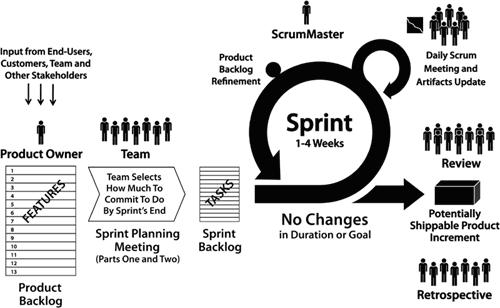
\includegraphics[width=\textwidth]{illustrations/scrum.jpg}
  \caption{An overview of SCRUM and its many activities. Of the displayed practices we have decided to use only the product backlog. Source: [\textit{http://softlinksolutions.com/development\_methodology.aspx}]}
  \label{scrum_picture}
\end{figure}

As just mentioned, we have decided to use a backlog, which is another SCRUM artifact.
The backlog is a prioritized list of items, where each item describes a program feature, often called a `story', possibly with sub-tasks that needs to be completed. Traditionally the product owner defines the order of the items, putting the features he wants implemented first at the top of the list \cite[p. 12]{scrum-org-guide}.
We have chosen to use a backlog as it ensures that the most vital functionality is implemented before less important, nice-to-have features. We will also benefit from producing the backlog itself, as we will be forced into enumerating all features to implement, giving us an overview of the work and ensuring that no big task suddenly pops up later.
Our complete backlog can be viewed in \atref{backlog}.

We have chosen not to divide our project into sprints, even though they are a core foundation of SCRUM.
Sprints are great for projects with longer time spans than ours, as it divides the project into smaller iterations, each producing valuable functionality able to function on its own, making it easier to keep focus.
After every sprint, the SCRUM team does a review, a retrospective, and plan which backlog items to implement during for the next sprint \cite[p. 8]{scrum-org-guide}.
Were we to divide our project into sprints, it would be very short ones, and it would not be worth the overhead from managing sprint backlogs and do reviews and retrospectives.

During a sprint, a SCRUM Task Board artifact is used to maintain overview of the sprint progress. The board is divided into four parts (`not started',`in progress', `to test' and `complete') with each task of the sprint listed under the appropriate section.
When a task is started it is moved from `not started' to `in progress', when a task is finished it is moved to `to test', and when it has passed its tests it is moved to `complete'.
Often a physical board is used so everyone, all the time, is able to keep track of the progress. This however, is only possible if all team members are at the same location, and it may be difficult to do, if the team cannot persist the board between sessions, for instance if the work location changes for each meeting.
For our project we have found a way to deploy a task board with minimum overhead by using a software version, always allowing every team member to keep track of the project wherever they are. Since we do not use sprints, the task board will give an overview of the progress of the whole project and of the individual tasks.\\
A sample of our task board can be viewed in figure \ref{taskboard} of the appendix.

The burndown chart in SCRUM (as well as in other measurable environments) is used to monitor the progress of remaining tasks - in SCRUM this is the sprint backlog.
The burndown chart is a basic diagram where the y-axis symbolizes the remaining work and the x-axis symbolizes the remaining time to complete the work.
When the sprint is started a diagonal line is drawn from $(0, y)$ to $(x, 0)$, where $y$ is the amount of work and $x$ is the amount of time.
Each day the progress is plotted in with a line, which shows the current status, and thereby maybe even the effectiveness of the team. If the latest progress line ends below or at the diagonal line, the project is progressing well; if not, the project is progressing too slowly, and the sprint will not be completed in time with all planned features.
Since our project effectively is a "one sprint"-project, we will use the burndown chart to measure whether we are on track or are falling behind schedule.\\
Our burndown chart at the time of writing can be viewed in figure \ref{burndown} of the appendix.

To perform and maintain the various artifacts described above, we have chosen to use scrumwise.com for all SCRUM related work. Our overhead from using SCRUM will be reduced, since the artifacts automatically will be updated whenever progress or changes are made to the backlog tasks.
Because the artifacts automatically are updated and always will be up to date, the site will easily allow us to monitor our progress and maintain our overview. Should our work not progress as estimated and planned, we will be able to spot it immediately, and may then pause our work to re-evaluate our plans, possible doing re-estimation of some or all of the tasks.
